\firstsection{Introduction}
\maketitle

% (What is the high level motivation)
% What is the obsatcle for effectively apply machine learning model
With the recent advances in neural network based model, machine learning has
gained unprecedented popularity, and its adaption permeated many fields of studies.
%
However, from researchers to practitioners, one often need to overcome many
obstacles during the training, debugging, and tuning processes to unleash
the full potential of these models.
%
Identify where and how does the error occur and come up with hypothesis for
why does the model fail is critical to the design and application of various models.
%quickly identify where the errors are
However, providing meaningful answers to these questions is an extremely challenging task.
% Naturally the identification of failure scenarios is an essential first step in diagnosing procedure.
%the potential limitation of the test dataset
On the one hand, recognize where the model fail is non-trivial. The standard evaluation approach (i.e., the prediction accuracy on the test set) provides limited information and cannot answer many important questions that are essential to the model diagnostic process. Questions such as, how stable predictions are concerning small perturbation in the input, how these predictions arrive (i.e., the model may come up with the correct prediction by pickup unintended feature/alignment), and what are the often made mistakes, are all essential in systematic examination and evaluation of the model. On the other hand, infer why the model fails is even more challenging. Since neural network models are often referred to as black boxes, hypothesizing what happened in prediction process require the ability to peek inside the model and understand the intricate relationships among model inputs, critical internal mechanisms, as well the output predictions.

\begin{itemize}
    \item Study the classifier  vs. single instance evaluation
    \item Model agnostic vs. reveal internal states
    \item View model as invariant object vs. interrogate the model via partial/full updates
\end{itemize}

%%%%%%%%% accessing internal states are important %%%%%%%%%%%%
Several previous works~\cite{BilalJourablooYe2018} have dedicate to analyzing errors made in analyzing 
There has been a
To analyzing the
Many method has been

The wide application of machine learning models also call for increasing demands for model accountability (e.g., what is the evidence for making the decision) and model fairness (e.g., is the prediction affected by the bias in the training data).
% Making sense and explaining predictions made by neural networks is also becoming a necessity.
%
Many works~\cite{RibeiroSinghGuestrin2016} have been dedicated to providing intuitive explanations for a given prediction, several of which approach the problem from a model agnostic approach that made them applicable to different applications (i.e., by fitting a simplier linear model near the prediction of interests).
%
Despite being invaluable for the providing human understandable explaination, the lack of the ability to access and explore the internal states of the model, which is vitally important to make sense of why a model fail, limits their ability for more in depth exploration and evaluation of the model.


%%%%%%%%%% interrogate relationship between different componenet, modified different componenets %%%%%%%%%%%
Beside looking into the internal states, understanding how each of the component of the model interact with input and output as well as with each other is the crucial for truly exmaine the mechanism of the model.
%
Look at how the model work in action and interrogate relationship between different component, i.e., how the change made to one part of model affect the other pieces present, is the key to gain the full picture.

\begin{figure}[htbp]
\centering
\vspace{-2mm}
 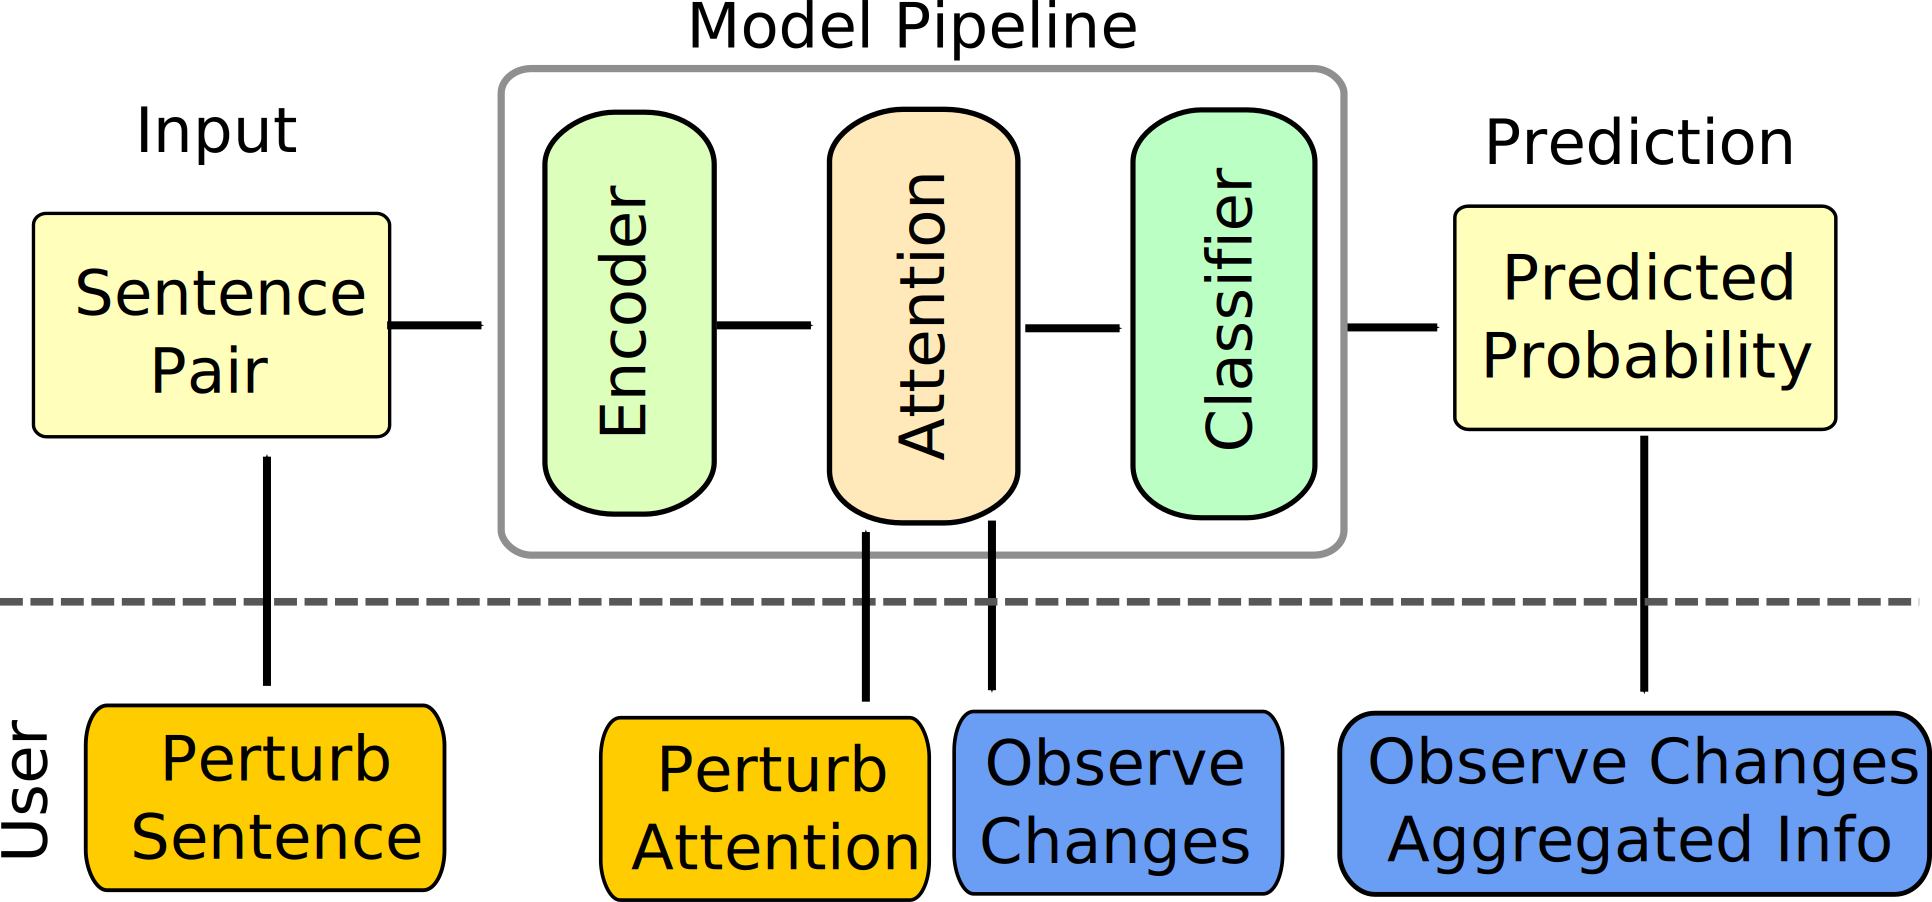
\includegraphics[width=1.0\linewidth]{pipeline}
 \caption{Language Inference Model Pipeline.}
\label{fig:projTransition}
\end{figure}

In this work, we introduce a visualization system that through a tight yet flexible integration between visual analytic elements and the underlying model, allow a user to interrogate the model by perturbing the input, the internal state, as well as prediction while observing changes in other parts of the pipeline.
We use natural language inference task~\cite{BowmanAngeliPotts2015} as an example to illustrate how this system help natural language processing (NLP) researchers quickly identify the potential limitation of an NLP model, probe the inner states of the model for interpreting key mechanism such as attention, and ultimately come up with hypothesis on why the model fails.

% ######## Why use perturbation ###########
% Iterate the model design and debug the system hinged on the ability to quickly
% identify the errors made by a model.
%
% Perturbe the input is what NLP researchers have subconsciously been doing to study and test a model.
%
% Interpret/probe the relationship between attention and the prediction result


The key contributions of the proposed works is summarized as the following:
\begin{itemize}
    \item Identify the mistakes made by the model through perturbation of input sentences and visual summarization of the predictions;

    \item Enhance the visual representation of attention by overlaying sentence linguistic structure to allow grammar guided simplification;

    \item Enable the interrogation of the relationship between input sentences, attention, and the prediction by interactively exploring how the change in one of these elements affect other parts of the model.

\end{itemize}
